\chapter{Обзор предметной области}
\label{chapter1}

\section{Теория оптимизации}
\label{optimization}

Рассмотрим различные способы постановки задачи оптимизации \cite{criteries, multievol, multicriteria, optimize}.
\subsection{Задача скалярной оптимизации}
Задача скалярной (однокритериальной) оптимизации может быть определена как задача максимизации
целевой функции $f(x): X\rightarrow \mathbb{R}$, где $X\subseteq W$ --- множество допустимых решений, содержащееся в пространстве решений $W$. Множество $X$ задается либо перечислением допустимых решений (в случае их конечного числа), либо некоторым набором ограничений. Таким образом, задача скалярной оптимизации имеет вид $f(x)\rightarrow\max, x\in X$. Решением скалярной задачи оптимизации является $x^*\in X: f(x^*)\geq f(x)$ для всех $x\in X$.

\subsection{Многокритериальная задача оптимизации}
Рассмотрим совокупность критериев $\varphi=(\varphi_1,\varphi_2,..,\varphi_m)$, заданных на пространстве $W$.  Отдельный критерий называют частным критерием выбора, а множества его возможных значений --- шкалой критерия. Рассматриваемая совокупность задает отображение $\varphi:W\rightarrow W'$, где $W'$ --- критериальное пространство, включающее в себя прямое произведение шкал критериев. Решение многокритериальной задачи оптимизации можно свести к поиску наиболее предпочтительной точки множества достижимых значений критериев $Y=\varphi(X)\in W'$. Формализация понятия наиболее предпочтительной точки может быть осуществлена, например, путем введения понятия доминирования по Парето. Заметим, что при решении многокритериальной задачи оптимизации в равной степени важны значения всех частных критериев.

\subsection{Задача оптимизации со вспомогательными критериями}
На практике возникает необходимость решать модифицированную скалярную задачу оптимизации, предполагающую наличие вспомогательных критериев. Она отличается от многокритериальной задачи тем, что целью ее решения по-прежнему является максимизация целевой функции, а вспомогательные критерии используются лишь для повышения эффективности процесса максимизации. В таких задачах целевая функция некоторым образом зависит от вспомогательных критериев, поэтому в некоторых случаях вместо максимизации целевой функции оказывается выгодным оптимизировать эти критерии.

Рассмотрим пример, в котором оптимизация по вспомогательным критериям оказывается выгодной. В работе \cite{master} возникает необходимость выбора между различными функциями приспособленности особей, представляющих тесты для проверки олимпиадных задач. В этом случае целевой функцией приспособленности, которую необходимо максимизировать, является время работы тестируемого решения.

\begin{figure}[h!]
\center{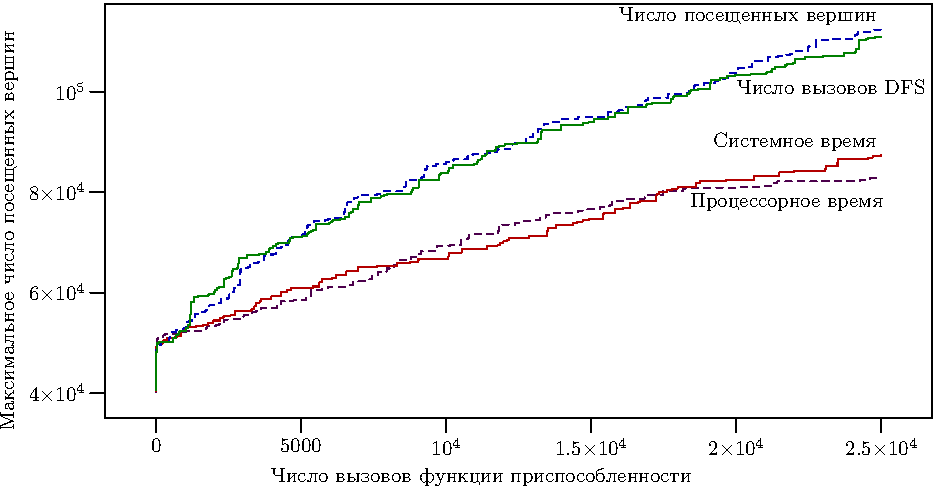
\includegraphics[width=\textwidth]{chart1}}
\caption{Сравнение функций приспособленности}
\label{pict:chart1}
\end{figure}

Оказывается, что время не является оптимальной функцией приспособленности. Предлагается использовать функции приспособленности, вычисляющие некий показатель сложности теста (например, число итераций алгоритма при прохождении теста). При оптимизации по этим вспомогательным функциям  удается получить тесты, время работы на которых на несколько порядков выше, чем значения, получаемые при оптимизации по самой целевой функции приспособленности. Подобное поведение проиллюстрировано на рис. \ref{pict:chart1}. Существует несколько вариантов таких вспомогательных функций, из которых также следует выбрать наиболее подходящий. Отметим новизну постановки задачи скалярной оптимизации, в которой фигурируют вспомогательные критерии.

Выбор между функциями приспособленности осуществляется вручную, что неэффективно, так как каждый запуск эволюционного алгоритма требует много ресурсов. Возникает задача автоматизации выбора функции приспособленности в течение одного запуска алгоритма оптимизации.


\section{Автоматическая настройка эволюционных алгоритмов}\label{ga}
В ходе работы предполагается автоматизировать выбор наиболее подходящей функции приспособленности. Рассмотрим, какие еще задачи автоматизации настройки эволюционных алгоритмов  решаются. К этим задачам относятся:
\begin{itemize}
  \item автоматическая настройка параметров (вероятностей мутации и кроссовера, размера поколения);
 	\item разработка адаптивных эволюционных операторов, таких как операторы мутации и кроссовера;
 	\item разработка адаптивных способов представления особей;
 	\item адаптивная настройка функций приспособленности.
\end{itemize}
Наиболее широко изучена автоматическая настройка параметров. Предлагаемая тема может быть отнесена к адаптивной настройке функций приспособленности, разработки по которой встречаются в литературе значительно реже. Предлагаемая постановка задачи отличается новизной, так как в других подобных исследованиях акцент делался на настройке некоторой фиксированной функции \cite{filtered-ff}. В разрабатываемом методе предлагается выбирать между качественно разными функциями.

\section{Машинное обучение}
\label{ml}	
	Методы машинного обучения \cite{mitchell-ml} предоставляют обобщенные подходы к решению задач, что позволяет применять их во многих областях: от разработки оптимальных стратегий игр и управления техническими процессами до решения задач распознавания и классификации. Рассмотрим основные подходы, применяющиеся в машинном обучении, с целью анализа их применимости к выбору вспомогательных функций приспособленности генетического алгоритма.
	\subsection{Деревья принятия решений и обучение концептам}
	Деревья принятия решений используются для классификации данных. Они позволяют аппроксимировать заданную булевскую функцию. Обучение ведется на конечных наборах дискретных атрибутов, для каждого из которых задано значение аппроксимируемой функции. Также для классификации данных в схожих условиях применяется обучение концептам \cite{mitchell-ml}.
	Требование наличия готового набора тестовых примеров, их дискретный характер, а также сама цель подобных методов, заключающаяся в классификации данных, затрудняют их применение к решению поставленной задачи.
	\subsection{Нейронные сети}	
	Помимо аппроксимации булевских функций и решения задач классификации, некоторые виды нейронных сетей позволяют аппроксимировать нелинейные функции с вещественными значениями. Большинство модификаций нейронных сетей предполагает наличие заранее подготовленного обучающего набора, хотя существуют подходы, позволяющие сделать обучение нейронной сети инкрементальным \cite{incremental}.
	Была предпринята попытка аппроксимации зависимости целевой функции приспособленности от дополнительных функций с помощью многослойной нейронной сети, составленной из нелинейных перцептронов и использующей алгоритм обратного распространения ошибки \cite{alpaydin, systems}. Также применялась реализация нейронной сети из библиотеки алгоритмов машинного обучения \emph{Encog}~\cite{encog}, в которой использовался алгоритм \emph{Quickprop} \cite{quickprop}. Эти нейронные сети показывали хорошие результаты аппроксимации несложных вещественных функций, но для решения поставленной задачи их точности не хватило. Однако дальнейшее исследование возможности использования нейронных сетей, особенно их инкрементальных модификаций, для выбора функций приспособленности кажется целесообразным.
	\subsection{Байесовское обучение}
	К методом байесовского обучения относятся, например, классификатор Гиббса и наивный байесовский классификатор \cite{mitchell-ml}. Они позволяют решать задачи классификации с большим количеством параметров. Обучаются на заранее подготовленных наборах тестовых примеров. Применение подобных методов для решения поставленной задачи затруднительно, так как ее сведение к задаче классификации неочевидно.
	\subsection{Алгоритмы кластеризации}
	Задача кластеризации \cite{alpaydin} возникает в анализе данных, распознавании образов, а также в биоинформатике, например, при выделении семейств генов, отвечающих за то или иное биологическое свойство. Алгоритмы кластеризации позволяют разделить объекты одной природы на несколько групп таким образом, чтобы объекты каждой группы были близки между собой, а объекты из разных групп существенно различались. Поставленная задача не относится к задачам кластеризации.
	
\section{Обучение с подкреплением}
	\label{rl}
	Большинство алгоритмов обучения с подкреплением \cite{sutton} не требует наличия заранее подготовленного набора тестовых примеров \cite{survey}. В алгоритмах этого типа обучение происходит одновременно с применением накопленного опыта, что позволяет выбирать и применять оптимальные ФП в течение одного запуска эволюционного алгоритма. Таким образом, обучение с подкреплением было выбрано в качестве используемого метода. Отметим новизну применения обучения с подкреплением к оптимизации эволюционных алгоритмов.
	
	Обучение с подкреплением решает задачу разработки стратегии поведения в интерактивной среде. Агент применяет действие к среде, после чего получает вещественнозначное вознаграждение и некоторое представление текущего состояния среды. Процесс обучения представляет собой последовательность таких взаимодействий, будем называть их шагами алгоритма обучения. Задачей агента является выработка стратегии поведения, приводящей к максимизации суммарного вознаграждения. Таким образом, для постановки \emph{задачи обучения с подкреплением} необходимо определить следующие компоненты:
	\begin{itemize}
		\item дискретное множество состояний среды, $S$;
		\item дискретное множество действий агента, $A$;
		\item множество возможных значений вознаграждения (сигналов);
		\item правило, по которому паре $(s \in S, a \in A)$ сопоставляется сигнал.
	\end{itemize}
	
	Схема обучения с подкреплением представлена на рис. \ref{rl-scheme}. Шаги на схеме нумеруются с помощью переменной $t$. Отметим, что для ряда алгоритмов обучения с подкреплением доказана сходимость к оптимальной стратегии максимизации вознаграждения \cite{systems}.
	
	\begin{figure}[h!]
	\center{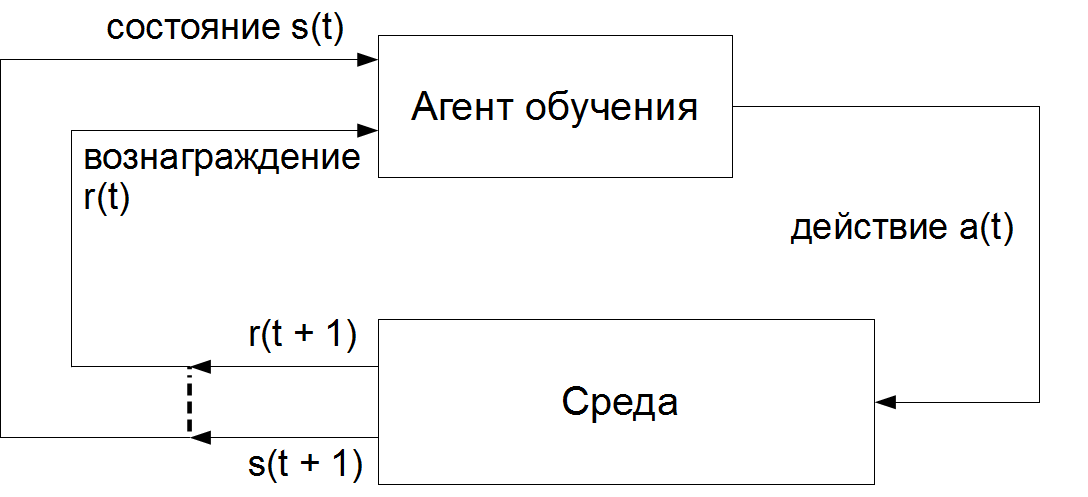
\includegraphics[width=0.6\textwidth]{rl-scheme}}
	\caption{Схема обучения с подкреплением}
	\label{rl-scheme}
	\end{figure}
		
		\subsection{Оценка оптимальности поведения агента}
		\label{mark}
		
		Для оценки оптимальности стратегии поведения агента применяются различные модели. Будем обозначать вознаграждение, полученное в результате $t$-ого взаимодействия агента со средой, как $r_t$. 
		
		В \emph{модели конечного горизонта} агент должен оптимизировать ожидаемую награду для следующих $h$ шагов:
		$$E(\sum_{t = 0} ^ {h} {r_t}).$$
		Эта модель применима, если число шагов алгоритма заранее известно. В общем случае время жизни агента не определено, поэтому модель конечного горизонта не получила широкого распространения \cite{survey}.
				
		\emph{Модель бесконечного горизонта} не ставит ограничений на количество шагов алгоритма. В ней следует максимизировать величину
		$$E(\sum_{t = 0}^{\infty}{\gamma^t r_t}).$$
		Здесь $0 \leq \gamma < 1$ -- дисконтный фактор, позволяющий учитывать, когда было получено вознаграждение. Больший вклад в награду вносят вознаграждения, полученные раньше. Эта модель является одной из самых популярных моделей оценки оптимальности поведения агента в алгоритмах обучения с подкреплением \cite{systems}.
		
		Также существует \emph{модель среднего вознаграждения}, в которой максимизируется предел ожидания среднего вознаграждения:
		$$\lim_{h \rightarrow 0} E(\frac{1}{h} \sum_{t=0}^{h}{r_t}).$$
		Эта модель, в отличие от модели бесконечного горизонта, не дает преимущества быстрой прибыли. В некоторых случаях она может быть более эффективна для решения поставленных задач \cite{average}. С другой стороны, существуют работы, в которых утверждается, что результаты, получаемые в модели среднего вознаграждения, могут быть столь же эффективно получены и в модели бесконечного горизонта \cite{average-discounted}. В настоящей работе алгоритм обучения R-learning \cite{r-learning}, основанный на модели среднего вознаграждения, показал наилучшие результаты в решении модельной задачи H-IFF \cite{mh-iff}, что описано в разд. \ref{h-iff-results}. 
		
		\subsection{Стратегии исследования среды}
		\label{strategy}
		
		 В обучении с подкреплением исследование среды (exploration) совмещается с применением накопленного опыта, заключающемся в следовании выработанной стратегии (exploitation) \cite{survey}. Существуют различные стратегии подобного совмещения. Простейшая \emph{жадная} стратегия состоит в том, чтобы всегда выбирать действие, ожидаемое вознаграждение за которое максимально. Следование этой стратегии может привести к тому, что агент выберет локально оптимальное поведение, недостаточно исследовав среду. 
		 
		 Жадную стратегию можно улучшить, выбирая с некоторой вероятностью $\varepsilon$ случайное действие, а с вероятностью $1 - \varepsilon$ --- по-прежнему действие, приводящее к максимальному ожидаемому вознаграждению. Такая стратегия носит название \emph{$\varepsilon$-жадной}. Значение $\varepsilon$ может уменьшаться со временем, что позволяет постепенно переходить от исследования среды к применению опыта. Подобная тактика наиболее эффективна в том случае, когда свойства среды не меняются.
		 
		 Также можно отметить \emph{исследование по Больцману} \cite{systems}, при котором вероятность выбора действия $a$ на текущем шаге определяется следующей формулой:
		 $$p(a) = \frac{e^{ER(a)/T}}{\sum_{a' \in A}{e^{ER(a')/T}}},$$
		где ER --- ожидаемое вознаграждение, Т --- температура, убывающий со временем параметр. Эта стратегия также наиболее эффективна в случае постоянной среды.
		 
		 В некоторых алгоритмах обучения с подкреплением применяются особые эвристики, определяющие выбор действия. Подробнее с различными стратегиями исследования среды можно ознакомиться в \cite{survey}.
		 
		\subsection{Марковский процесс принятия решений} 
		В общем случае действие агента определяет не только получаемое вознаграждение, но и состояние, в которое переходит среда после воздействия. Таким образом, возникает понятие отложенного вознаграждения. Возможна стратегия, в соответствии с которой агент должен в течение некоторого времени получать незначительное вознаграждение, чтобы в итоге достичь состояния среды, которому соответствует большое вознаграждение. Задачи обучения с подкреплением в случае отложенного вознаграждения могут быть описаны как \emph{Марковский процесс принятия решений} (МППР) \cite{systems, sutton}. МППР определяют следующие компоненты:
		\begin{itemize}
		  \item дискретное множество состояний среды $S$;
		  \item дискретное множество действий агента $A$;
		  \item функция вознаграждения $R : S\times A \rightarrow \mathbb{R}$
		  \item функция переходов $T : S\times A\times S\rightarrow \mathbb{R}$ 
				такая, что вероятность перехода из состояния $s$ в состояние $s'$ в результате воздействия $a$ задается значением $T(s, a, s').$
		\end{itemize}
		
		\subsection{Q-обучение}
		Опишем Q-обучение --- алгоритм обучения с подкреплением, не строящий модель среды и относящийся к семейству алгоритмов итерации по значениям \cite{ii, systems, sutton}. В ходе работы этого алгоритма аппроксимируется функция $Q(s, a), s \in S, a \in A$ --- ожидаемое оптимальное вознаграждение за действие $a$ в состоянии $s$. В качестве стратегии исследования среды будем использовать $\varepsilon$-жадную стратегию. В листинге \ref{ql} приведен псевдокод алгоритма.
		
		\begin{algorithm}[h!]
		\caption{Алгоритм Q-обучения с $\varepsilon$-жадной стратегией исследования среды}
		\label{ql}
		%{\fontsize{12}{12}\selectfont
		\begin{algorithmic}[1]
		\REQUIRE  
			$\varepsilon$ --- вероятность выбора случайного действия;
			$\alpha$ --- скорость обучения;
			$\gamma$ --- дисконтный фактор.
		\STATE {Инициализировать $Q(s, a)$ для всех $s \in S$, $a \in A$}
		\WHILE{{(не достигнуто условие останова)}}
			\STATE {Получить состояние среды $s$}
			\STATE $p \gets ${ случайное вещественное число} $\in [0, 1]$
			\IF {($p \leq \varepsilon$)}
				\STATE $a \gets \arg \max_{a}{Q(s,a)}$
			\ELSE 
				\STATE $a \gets$ { случайное действие } $\in A$
			\ENDIF
			\STATE {Применить действие $a$ к среде}
			\STATE {Получить от среды награду $r$ и состояние $s'$}
			\STATE $Q(s,a) \gets Q(s,a) + \alpha(r + \gamma \max_{a'}{Q(s',a') - Q(s, a))}$
		\ENDWHILE
		\end{algorithmic}
		%}
		\end{algorithm}
		
		Отметим, что существует алгоритм отложенного Q-обучения, Delayed Q-learning, для которого доказана более высокая скорость сходимости \cite{delayed}. Этот алгоритм, как и алгоритм Q-обучения, был реализован в рамках настоящей работы.
		
		Также в данной работе использовался алгоритм Dyna \cite{sutton}, относящийся к классу алгоритмов, строящих модель среды. Такие алгоритмы аппроксимируют и используют для определения стратегии поведения функцию вознаграждения $R$ и функцию переходов $T$. В применении к рассматривавшимся модельным задачам алгоритм Dyna не показал высоких результатов.

\section{Выводы по главе \protect\ref{chapter1}}
Описаны задачи скалярной и многокритериальной оптимизации. Поставлена задача скалярной оптимизации со вспомогательными критериями. Она возникает на практике при использовании эволюционных алгоритмов и наличии набора вспомогательных функций приспособленности. Отмечена новизна постановки задачи. 

Обоснована необходимость разработки метода автоматизации выбора вспомогательных функций приспособленности. Рассмотрены другие подходы к автоматизации эволюционных алгоритмов. Рассмотренные подходы не позволяют решить поставленную задачу. 

Обоснован выбор методов машинного обучения в качестве основы разрабатываемого метода. Произведен обзор методов машинного обучения. Обоснована применимость обучения с подкреплением к решению поставленной задачи. Отмечена новизна применения обучения с подкреплением к оптимизации производительности эволюционных алгоритмов.

Кратко описана теория обучения с подкреплением, которое применяется для разработки стратегии поведения агента в интерактивной среде. Формализована задача обучения с подкреплением. Определены способы оценки оптимальности поведения агента. Перечислены наиболее часто использующиеся стратегии совмещения исследования среды с применением накопленного опыта. Дано понятие Марковского процесса принятия решений, которому соответствует типичная задача обучения с подкреплением. Описано Q-обучение --- один из базовых алгоритмов обучения с подкреплением, не строящих модель среды.

\label{summary_1}

